\section{Tauri}
\label{sec:tauri}
Tauri was first released at \displaydate{dateTauriRelease}~\cite{tauriRelease} and downloaded approx. $58\,000$ times\footnote{According to \url{https://npm-stat.com/charts.html?package=tauri&from=2019-12-31&to=2022-08-12}}.
It resulted as discontent of Electron from the Tauri Developers especially in case of resource consumption and security due to uncontrollable dependencies.
They criticized the enormous resource consumption even of the simplest applications as well as the fact, that Electron does not have control over their dependencies.
If Chromium encounters a zero-day-exploit and releases a patch, Electron has to include this patch and also release a newer versions.
This leads to the fact, that users of an Electron-based application have to update their whole electron version to close this security issue.
This timespan, between first fix of chromium and the users update of the applications, is a high vulnerability for attackers.
In this regard, the developers also criticized the power of the privileges Electron applications have, allowing attackers to have access to the entire hard drive of the user for example~\cite{tauri}.
But like Electron Tauri experienced increased attention, which as in~\ref{sec:electron} can be expressed numerically based on GitHub Statistics~\cite{GithubTauri}: \\ \\
\begin{tabular} {| c | c | c | c | c |}
    \label{tab:tauri:statistics}
    Stars      & Forks     & Watching & Used by    & Contributors \\ \hline
    $48\,200$ & $1\,200$ & $403$ & $3\,200$ & $182$
\end{tabular} \\ \\
But unlike Electron, Tauri uses the self developed core, called Tauri, which is written in Rust in combination with WRY, which serves as the rendering library.


\subsection{Architecture}
\label{subsec:tauri:architecture}
The architecture of Tauri is very similar to Electrons multiprocess model.
Tauri also relies on a main process, called \textbf{core} process and multiple rendering processes, called \textbf{webview} for performance as well as security reasons.
\figref{fig:tauri:model} shows the basic architecture of Tauris multiprocess model whereas each \texttt{webview} process is managed by the \texttt{core} process.
by the
\begin{figure}[ht]
    \centering
    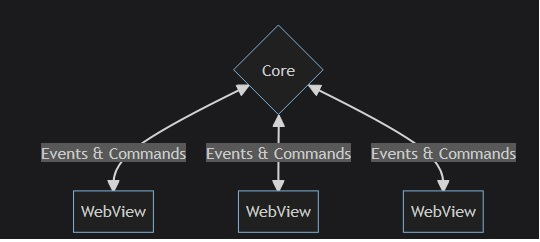
\includegraphics[width=0.4\textwidth]{images/TauriArchitecture}
    \caption{Multi-process Model Tauri from~\cite{tauri}}
    \label{fig:tauri:model}
\end{figure}

\begin{description}
    \item[\textbf{Core}:] \hfill \\ This is the main entry point of the application and the only place where full access to the operating system is provided.
    The \texttt{core} process uses this privileges to create and manage the windows the application.
    But it is also the only point, where the communication between processes is going through, allowing the core process to manipulate or observe \ac{IPC} messages.
    Additional the \texttt{core} process is responsible for global scoped cases such as database access or managing application or os-specific settings that affect the windows.
    Summarized it serves as a centralized management and control point, where the application as itself is maintained and sensitive data is kept to be hidden from the \texttt{webview} processes.


    \item[\textbf{WebView}:] \hfill \\ A \texttt{webview} process renders the ui by using the WebView libraries of the current os.
    Since this library is not included into the final executable but linked at runtime, it differs depending on the operating system the application is executed.
    This reduces the size of the executable since the part where the actual rendering takes places is shifted from the application to the operating system but also results
    that developers have to keep in mind the different operating systems.

\end{description}

\subsubsection{Inter Process Communication}
For communication between different processes Tauri also uses Inter Process Communication similar to Electron.
In contrast, Tauri forces developers from the beginning to use the \ac{AMP} paradigm, whereas Electron released this feature at version 14 and only recommends it.
The main advantage of \ac{AMP} is, that direct function access is denied and thus all communication has to go through the \texttt{core} process.
Since it is able to observe the content of messages, it can decide which message will be forwarded and which will be blocked like malicious requests.
Communication can be either unidirectional using events, which can be emitted by both \texttt{core} and \texttt{webview} processes to inform the event recipient but without any response,
or using commands which are bidirectional \ac{IPC} messages but can only be emitted by the \texttt{webview} processes to invoke functions that require access to the operating system.

\subsubsection{Context Isolation}
In contrast to Electron Tauri uses different patterns for isolating critical \ac{API} calls communication between the \texttt{webview} processes and the \texttt{core} process.
They are called Brownfield and Isolation Pattern, whereas the default pattern, that can be configured inside the \texttt{tauri.conf.json} is the Brownfield pattern
\begin{description}
    \item[\textbf{Brownfield Pattern}:] \hfill \\
    The Brownfield pattern can be seen as a design pattern to ensure interoperability between new implemented and existing software.
    This pattern does not categorize software as legacy software but as current state of the art and software developed following this pattern tries to coexist and consider existing software as much as possible.
    This requires a deep knowledge of the existing software and also can result in re-developing significant parts of the existing software when tried to enhance new features.
    Tauri uses this pattern as standard and explains that it tries to be as compatible as possible.
    But unfortunately Tauri does not explain in detail how they are implementing this pattern and how this helps to avoid malicious frontend calls to the Tauri core~\cite{tauri}.
    \item[\textbf{Isolation Pattern}:] \hfill \\
    The Isolation Pattern can be seen as an interposed instance between the \ac{IPC} handler and the processes.
    This instance is providing a sandbox, called Isolation application, which is trusted and secure JavaScript code embedded into an \texttt{<iframe>}.
    The \ac{IPC} handler passes its message to the Isolation application, where it is executed and may be modified or verified.
    After that it will be encrypted, passed back to the \ac{IPC} handler and forwarded to the \texttt{core} process, where it will be handled as normal.


\end{description}

\begin{figure}[ht]
    \centering
    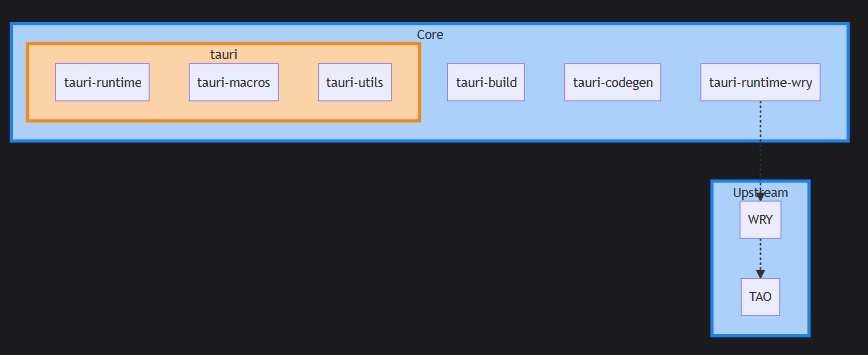
\includegraphics[width=0.4\textwidth]{images/TauriCore}
    \caption{Core Ecosystem from~\cite{tauri}}
    \label{fig:tauri:core}
\end{figure}
As it can be seen in \figref{fig:tauri:core} Tauri splits its framework into two main components.
The Core, containing several modules providing API access, utilities and the runtime.
The Upstream containing the two self-developed Rust crates WRY and TAO which are providing libraries for creation and rendering of WebViews and their content.
%Same as described for Tauri.Ref to introduction\ref{subsec:electron:arch}

\subsection{Frontend}
\label{subsec:tauri:frontend}
As mentioned above, Tauris frontend relies on its own implementation of WebView instead of the entire Chromium content module for rendering \ac{HTML} content.
This makes it much smaller than electron applications since their libraries WRY and TAO are using the exising web engines of the three major operating systems Linux, macOS and Windows instead of shipping an entire browser.
\begin{description}
    \item[\textbf{TAO}:] \hfill \\
    TAO is a cross-platform library written in Rust and used for creating and managing application windows.
    It was forked from the Rust crate \texttt{winit} since the developers wanted to enhance more desktop features than the original crate, like menu bars or a system tray.
    This library ships with an entire event loop that can be emitted by windows like resizing or key interactions and is included at the second frontend library WRY.
    \item[\textbf{WRY}:] \hfill \\
    WRY is the main library at Tauri application and responsible for rendering the content of the os-specific web view.
    It acts as an interface between the Tauri core with its low level webview drivers and the webview technology of the current operating system, providing an unique abstraction layer for rendering webview content.
    Since it re-exports TAO and its event loop to guarantee access to os-specific web engines the appearance of the same application may differ on each operating system, depending on the underlying web engine.
\end{description}
%WRY and TAO
%Webview implementierung
\subsection{Backend}
\label{subsec:tauri:backend}
The backend or core of Tauri contains of several components, whereas some of them are summarized and called \texttt{tauri} to emphasize the main part of each Tauri application including runtime or the Tauri \ac{API}.
The decision to write the entire backend in Rust was made because of the ownership feature in Rust which provides a set of rules for memory management and avoiding a garbage collector like Java or explicit memory allocation like C.
It can be seen as an approach of trying to be more comfortable for the developer as an explicit allocation but also to force the developer to consider his/her memory handling to implement an efficient app.
This set of rules is checked at compile time and if one of them is violated, the program will not compile.
Beside that \texttt{tauri} components there are also additional components included by the core like system-level interactions for the upstream crate WRY .
One of the major advantages of using Rust for the Tauri backend is as already mentioned its ownership rules, avoiding security issues but also the execution time of Rust code which was intended to obtain a similar performance as C++.
Furthermore, Rust experienced a significant attention resulting in the adoption of it by big companies like Google or Facebook which assumes an increasing position.

TAURI CORE
ownership

